\section{Hardware supported multithreading}
I threads hanno PC, stack e registri del processore privati ma condividono la memoria (a differenza dei processi). Nella gestione dei thread non serve duplicare gran parte del processore, perchè le unità funzionali possono essere condivise. Ciò significa che i threads competono realmente per la stessa unità funzionale, e la memoria virtuale tramite i meccanismi di paging on demand fornisce un supporto enorme per gestire la memoria condivisa in termini di efficienza di spazio. Il cambiamento di contesto tra più threads è quasi immediato. Questo permette rapidi cambi di contesto in caso di eventi di stallo (come cache misses) per nascondere lunghe latenze. In questo caso stiamo parlando di Thread level parallelism (\textbf{TLP}), ed è gestito esplicitamente dal programmatore o dal compilatore. 
Possiamo identificare, in termini di sprechi di risorse del processore, \textit{sprechi} verticali e \textit{sprechi} orizzontali.

\begin{figure}[ht]
    \centering
    \setlength{\fboxrule}{0.5pt} % spessore sottile
    \setlength{\fboxsep}{0pt}    % senza spazio interno
    \fbox{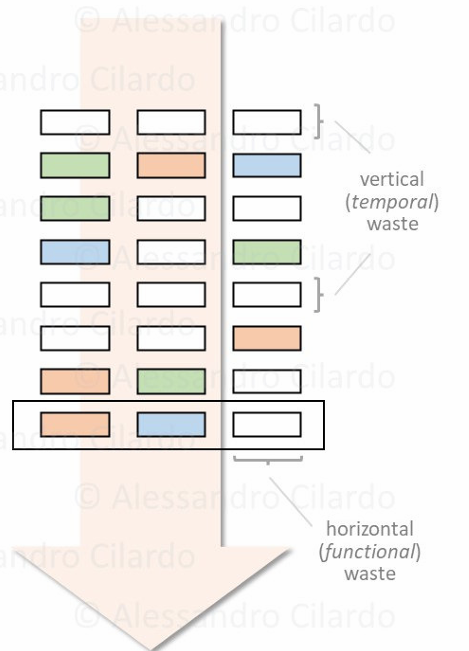
\includegraphics[width=0.6\textwidth]{fig/chapter_2/wasting.png}}
\end{figure}

Il meccanismo del multithreading simultaneo conviene perchè è possibile aumentare l'ampiezza della finestra di istruzioni recuperata (poichè i thread utilizzano istruzioni indipendenti) invece che la profondità. Si possono recuperare e accettare n istruzioni per colpo di clock, l'esecuzione è out of order e poi si possono committare fino a n istruzioni per clock. Questo risolve il problema della multiple issue. Vediamo con ordine le varie tipologie di hardware multithreading:

\begin{itemize}
    \item \textbf{Coarse-grain}: viene effettuato il cambio di contesto solo su eventi di attesa prolungata (come cache miss), e in generale su eventi che provocano sprechi verticali;
    \item 
\end{itemize}

